\documentclass[10pt]{article}
\usepackage{lmodern}
\usepackage[top=2.54cm, bottom=2.54cm, left=2.54cm, right=2.54cm]{geometry}
\usepackage{amsmath}
\usepackage{wrapfig}
\usepackage{tabularx}
\usepackage{graphicx}
\usepackage[inline]{enumitem}
\usepackage{fontawesome}
\usepackage[x11names]{xcolor}

\usepackage{hyperref}
\hypersetup{
  colorlinks=true,
  linkcolor=Black,
  urlcolor=RoyalBlue3
}
\usepackage{array} 

\usepackage{enumitem}
\setlist{nolistsep}

\usepackage{fancyhdr}
\pagestyle{fancy}
\fancyhf{}
\renewcommand{\headrulewidth}{0pt}
\lfoot{David \v{C}ern\'{y}}
\cfoot{Page \thepage\ of 5}
\rfoot{\textit{Curriculum vitae}}

\begin{document}
\frenchspacing

\begin{center}
{\LARGE \textsc{David \v{C}ern\'{y}}}

\begin{tabularx}{\textwidth}{c}
\hline
\end{tabularx}
\end{center}

\begin{center}
\begin{tabular}{l}
Henry Hinds Laboratory \\
5734 South Ellis Avenue \\
Chicago, IL 60637-1468 \\
\end{tabular}
\hfill
\begin{tabular}{rc}
\href{mailto:davidcerny@uchicago.edu}{davidcerny@uchicago.edu}  & \textcolor{RoyalBlue3}{\faEnvelope} \\
\href{http://davidcerny.github.io}{davidcerny.github.io} & \textcolor{RoyalBlue3}{\faUser} \\
\href{https://github.com/davidcerny}{github.com/davidcerny} & \textcolor{RoyalBlue3}{\faGithub} \\
\end{tabular}
\end{center}

\section*{Education}

\begin{tabularx}{\textwidth}{>{\raggedleft\arraybackslash}p{2.2cm} l}
2018--Present & Ph.D. candidate in Geophysical Sciences; University of Chicago \\[0.1cm]
2014--2018 & B.S. (Honors) in Ecology, Behavior, and Evolution; University of California, Los Angeles
\end{tabularx}

\section*{Research Experience}

\subsection*{Fall 2018--Present: Slater Lab}

\begin{tabularx}{\textwidth}{>{\raggedleft\arraybackslash}p{3.6cm} X}
Affiliation: & Department of the Geophysical Sciences, University of Chicago \\[0.1cm]
Position: & Ph.D. candidate \\[0.1cm]
Ph.D. advisor & Graham J. Slater
\end{tabularx}

\subsection*{Winter 2022--Spring 2022: Jablonski Lab}

\begin{tabularx}{\textwidth}{>{\raggedleft\arraybackslash}p{3.6cm} X}
Affiliation: & Department of the Geophysical Sciences, University of Chicago \\[0.1cm]
Position: & Research assistant \\[0.1cm]
Principal investigator: & David Jablonski \\[0.1cm]
Project: & Inferring a taxonomically comprehensive molecular phylogeny of cardiid bivalves
\end{tabularx}

\subsection*{Fall 2015--Summer 2018: Alfaro Lab}

\begin{tabularx}{\textwidth}{>{\raggedleft\arraybackslash}p{3.6cm} X}
Affiliation: & Department of Ecology and Evolutionary Biology, University of California, Los Angeles \\[0.1cm]
Position: & Undergraduate research assistant \\[0.1cm]
Principal investigator: & Michael E. Alfaro \\[0.1cm]
Projects: & Phylogenomic divergence dating of vertebrates; Exploration of form-function mapping using a \textsf{C++} simulation of polygenic trait evolution
\end{tabularx}

\subsection*{Winter 2018: Field \& Marine Biology Quarter in Mo'orea}

\begin{tabularx}{\textwidth}{>{\raggedleft\arraybackslash}p{3.6cm} X}
Affiliation: & Department of Ecology and Evolutionary Biology, University of California, Los Angeles \\[0.1cm]
Position: & Undergraduate student \\[0.1cm]
Principal investigator: & Daniel T. Blumstein \\[0.1cm]
Project: & Applying Lanchester's laws to the interspecific competition of coral reef fish
\end{tabularx}

\subsection*{Summer 2017: Kondrashov Lab}

\begin{tabularx}{\textwidth}{>{\raggedleft\arraybackslash}p{3.6cm} X}
Affiliation: & Evolutionary Genomics Group, Centre de Regulaci\'{o} Gen\`{o}mica (Centre for Genomic Regulation), Barcelona, Spain \\[0.1cm]
Position: & Research intern \\[0.1cm]
Principal investigators: & Fyodor Kondrashov, Dinara Usmanova \\[0.1cm]
Project: & Detecting positive selection using molecular phylogenies \\[0.1cm]
\end{tabularx}

\section*{Publications}

\subsection*{Peer-reviewed publications}

\begin{center}
  \begin{itemize*}
    \item 212 citations \hspace*{1cm}
    \item h-index: 4 \hspace*{1cm}
    \item i10-index: 4 \hspace*{1cm}
    \item \href{https://scholar.google.com/citations?user=LFXFNAMAAAAJ}{Google Scholar profile}
  \end{itemize*}
\end{center}

\noindent \begin{tabularx}{\textwidth}{>{\raggedleft\arraybackslash}p{2.2cm} X}
2023 & \textbf{\v{C}ern\'{y} D}, van Els P, Natale R, Gregory SMS. A new genus-group name for \textit{Burhinus bistriatus} (Wagler, 1829) and \textit{Burhinus superciliaris} (Tschudi, 1843). \textit{Avian Systematics} 1(3): 31--43.
\end{tabularx}

\begin{wrapfigure}{r}{0.18\textwidth}
 \begin{center}
   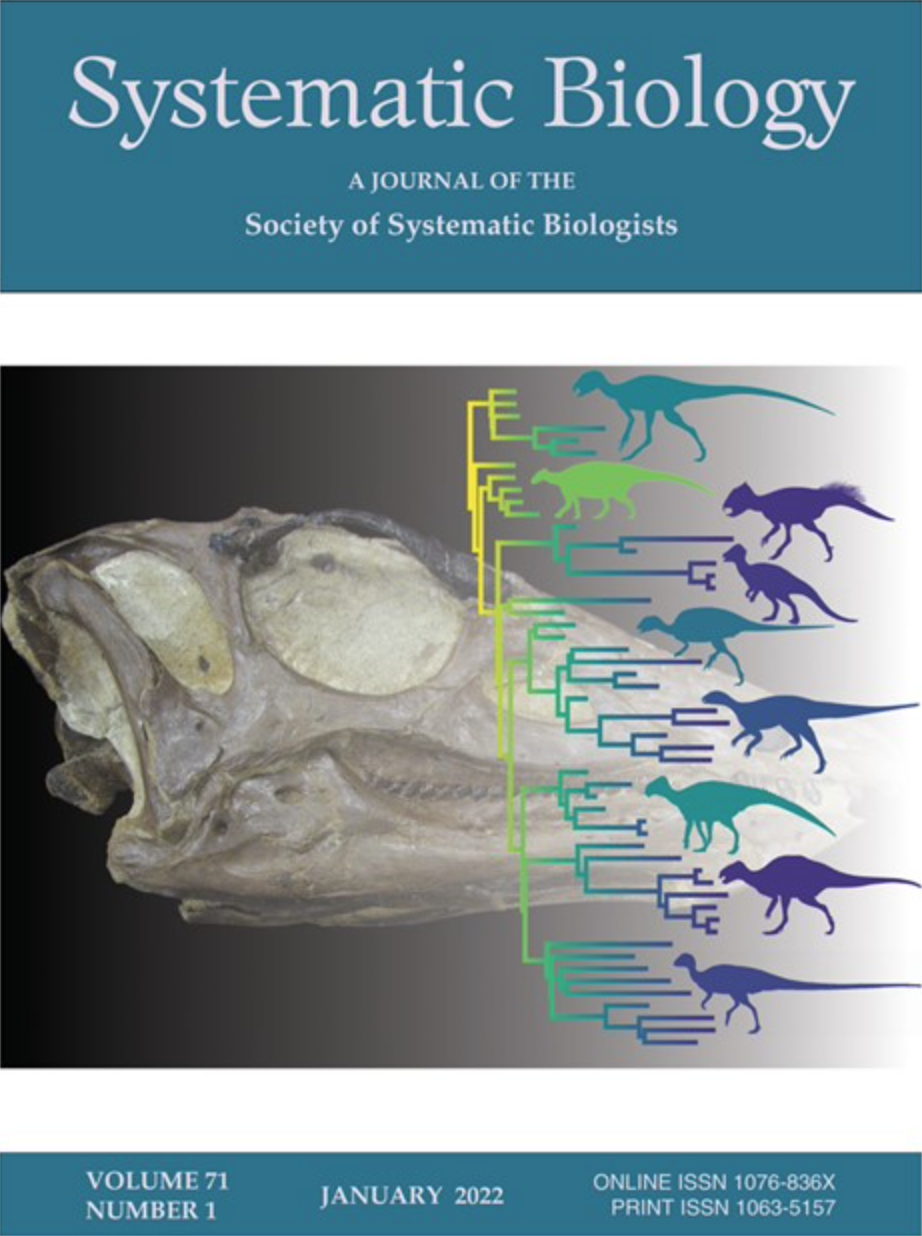
\includegraphics[width=0.16\textwidth]{SysBioCover.png}
 \end{center}
\end{wrapfigure}

\noindent \begin{tabularx}{\textwidth}{>{\raggedleft\arraybackslash}p{2.2cm} X}
2022 & \textbf{\v{C}ern\'{y} D}, Natale R. Comprehensive taxon sampling and vetted fossils help clarify the time tree of shorebirds (Aves, Charadriiformes). \textit{Molecular Phylogenetics and Evolution} 177: 107620. \href{http://doi.org/10.1016/j.ympev.2022.107620}{doi:10.1016/j.ympev.2022.107620}
\end{tabularx}
\begin{tabularx}{\textwidth}{>{\raggedleft\arraybackslash}p{2.2cm} p{10.5cm}}
2021 & \textbf{\v{C}ern\'{y} D}, Madzia D, Slater GJ. Empirical and methodological challenges to the model-based inference of diversification rates in extinct clades. \textit{Systematic Biology} 71(1): 153--171. \href{http://doi.org/10.1093/sysbio/syab045}{doi:10.1093/sysbio/syab045} (cover article)
\end{tabularx}
\begin{tabularx}{\textwidth}{>{\raggedleft\arraybackslash}p{2.2cm} p{10.5cm}}
2019 & Friedman M, Feilich KL, Beckett HT, Alfaro ME, Faircloth BC, \textbf{\v{C}ern\'{y} D}, Miya M, Near TJ, Harrington RC. Ancient adaptive radiation in the open ocean: rapid divergence in Pelagiaria (Acanthomorpha: Percomorpha) near the Cretaceous-Palaeogene boundary. \textit{Proceedings of the Royal Society B} 286(1910): 20191502. \href{http://doi.org/10.1098/rspb.2019.1502}{doi:10.1098/rspb.2019.1502}
\end{tabularx}
\begin{tabularx}{\textwidth}{>{\raggedleft\arraybackslash}p{2.2cm} X}
2018 & \textbf{\v{C}ern\'{y} D}, Lee K, Medal J, Blumstein DT. Applying Lanchester's laws to the interspecific competition of coral reef fish. \textit{Behavioral Ecology} 30(2): 426--433. \href{http://doi.org/10.1093/beheco/ary182}{doi:10.1093/beheco/ary182}
\end{tabularx}
\begin{tabularx}{\textwidth}{>{\raggedleft\arraybackslash}p{2.2cm} X}
2018 & Lima MGM, de Sousa e Silva-J\'{u}nior J, \textbf{\v{C}ern\'{y} D}, Buckner JC, Aleixo A, Chang J, Zheng J, Alfaro ME, Martins A, Di Fiore A, Boubli JP, Lynch Alfaro JW. A phylogenomic perspective on the robust capuchin monkey (\textit{Sapajus}) radiation. \textit{Molecular Phylogenetics and Evolution} 124: 137--50. \href{http://doi.org/10.1016/j.ympev.2018.02.023}{doi:10.1016/j.ympev.2018.02.023}
\end{tabularx}
\begin{tabularx}{\textwidth}{>{\raggedleft\arraybackslash}p{2.2cm} X}
2018 & Alfaro ME, Faircloth BC, Harrington RC, Sorenson L, Friedman M, Thacker CE, Oliveros CH, \textbf{\v{C}ern\'{y} D}, Near TJ. Explosive diversification of marine fishes at the Cretaceous-Paleogene boundary. \textit{Nature Ecology and Evolution} 2: 688--96. \href{http://doi.org/10.1038/s41559-018-0494-6}{doi:10.1038/s41559-018-0494-6}
\end{tabularx}

\subsection*{Manuscripts in review \& preprints}

\begin{tabularx}{\textwidth}{>{\raggedleft\arraybackslash}p{2.2cm} X}
In revision & \textbf{\v{C}ern\'{y} D}, Simonoff AL. Statistical evaluation of character support reveals the instability of higher-level dinosaur phylogeny. Available as a bioR$\chi$iv preprint: \href{https://www.biorxiv.org/content/10.1101/2023.01.25.525612v1}{doi:10.1101/2023.01.25.525612 }
\end{tabularx}

\subsection*{Other publications}

\begin{tabularx}{\textwidth}{>{\raggedleft\arraybackslash}p{2.2cm} X}
2020 & \textbf{\v{C}ern\'{y} D}. Palaeontology's greatest ever graphs:
Stadler's sampled tree: \textit{The Palaeontology Newsletter} 105: 63--65.
\end{tabularx}
\begin{tabularx}{\textwidth}{>{\raggedleft\arraybackslash}p{2.2cm} X}
2018 & \textbf{\v{C}ern\'{y} D}. [Review of] \textit{Birds of Stone: Chinese Avian Fossils from the Age of Dinosaurs}. \textit{Fossil News}, Summer 2018: 23--27.
\end{tabularx}

\section*{Presentations \& Posters}

\subsection*{Invited presentations}

\begin{tabularx}{\textwidth}{>{\raggedleft\arraybackslash}p{2.2cm} X}
2022 & \textbf{\v{C}ern\'{y} D*}, Schwery O. Inferring diversification rates from fossil data: assumptions, choices, challenges. Evolution, June 24--28, Cleveland, OH. (Symposium talk)
\end{tabularx}

\subsection*{Contributed presentations}

\begin{tabularx}{\textwidth}{>{\raggedleft\arraybackslash}p{2.2cm} X}
2023 & \textbf{\v{C}ern\'{y} D*}, Slater GJ. Bayesian Least-Squares Supertrees (BLeSS): a flexible method for inferring large time-calibrated phylogenies. Society of Systematic Biologists Standalone Meeting, January 14--15, Ciudad de M\'{e}xico, Mexico. (Poster)
\end{tabularx}
\begin{tabularx}{\textwidth}{>{\raggedleft\arraybackslash}p{2.2cm} X}
2022 & \textbf{\v{C}ern\'{y} D*}. Relative impact of character coding differences and stratigraphic information on the support for alternative early dinosaur phylogenies. GSA Connects, October 9--12, Denver, CO. \href{ https://doi.org/10.1130/abs/2022AM-381871}{doi:10.1130/abs/2022AM-381871}
\end{tabularx}
\begin{tabularx}{\textwidth}{>{\raggedleft\arraybackslash}p{2.2cm} X}
2021 & Schwery O*, \textbf{\v{C}ern\'{y} D}. Investigating mammal/dung beetle co-diversification. Entomology Annual Meeting, October 31--November 3, Denver, CO. (On-demand virtual talk)
\end{tabularx}
\begin{tabularx}{\textwidth}{>{\raggedleft\arraybackslash}p{2.2cm} X}
2021 & \textbf{\v{C}ern\'{y} D*}, Natale R. Vetted calibrations and comprehensive taxon sampling clarify the timescale of shorebird evolution. Evolution, June 21--25, online. (Faux-live talk)
\end{tabularx}
\begin{tabularx}{\textwidth}{>{\raggedleft\arraybackslash}p{2.2cm} X}
2019 & \textbf{\v{C}ern\'{y} D*}, Madzia D, Slater GJ. Evaluating the performance of diversification rate estimation methods in extinct clades with empirical and simulated data. 3rd Annual Great Lakes Student Paleoconference, November 8--10, Ann Arbor, MI.
\end{tabularx}
\begin{tabularx}{\textwidth}{>{\raggedleft\arraybackslash}p{2.2cm} X}
2019 & \textbf{\v{C}ern\'{y} D*}, Madzia D, Slater GJ. Inferring macroevolutionary dynamics of extinct clades: a test using `bird-hipped' dinosaurs (Ornithischia). Evolution, June 21--25, Providence, RI.
\end{tabularx}
\begin{tabularx}{\textwidth}{>{\raggedleft\arraybackslash}p{2.2cm} X}
2018 & \textbf{\v{C}ern\'{y} D*}, Lee K, Medal J, Blumstein DT. A fish eat fish world: Applying Lanchester's laws of combat to the interspecific competition of coral reef fish. 21st UCLA Annual Biology Research Symposium, May 23, Los Angeles, CA. (Poster)
\end{tabularx}
\begin{tabularx}{\textwidth}{>{\raggedleft\arraybackslash}p{2.2cm} X}
2016 & \textbf{\v{C}ern\'{y} D*}, Alfaro ME. Phylogeny and divergence times of tetraodontiform fishes based on a new multi-locus dataset. 19th UCLA Annual Biology Research Symposium, May 11, Los Angeles, CA. (Poster, Honorable mention)
\end{tabularx} \\[1ex]

\hspace*{1.07cm} * Presenting author.

\section*{Fellowships \& Awards}

\begin{tabularx}{\textwidth}{>{\raggedleft\arraybackslash}p{2.2cm} X}
2018--Present & Neubauer Family Distinguished Doctoral Fellowship. (Neubauer Family Foundation) \\[0.1cm]
Spring 2022 & SSB Graduate Student Research Award. \textit{Bayesian inference of large-scale fossil time trees using a novel supertree method.} (Society of Systematic Biologists). \$3,000 \\[0.55cm]
2014--2018 & Bakala Foundation Scholarship. (Bakala Foundation) \\[0.1cm]
Summer 2016 & Whitcome Undergraduate Summer Research Fellowship. \textit{Inferring the evolutionary timescale of tetraodontiform fishes (Acanthomorpha: Eupercaria).} (Department of Ecology and Evolutionary Biology, UCLA). \$3,000
\end{tabularx}

\subsection*{Travel awards}

\begin{tabularx}{\textwidth}{>{\raggedleft\arraybackslash}p{2.2cm} X}
Winter 2023 & SSB Standalone Meeting Travel Award (Society of Systematic Biologists). \$500
\end{tabularx}
\begin{tabularx}{\textwidth}{>{\raggedleft\arraybackslash}p{2.2cm} X}
Winter 2018 & A. R. Wallace Scholarship for International Field and Marine Research. (Department of Ecology and Evolutionary Biology, UCLA). \$350
\end{tabularx}

\section*{Teaching}

\begin{tabularx}{\textwidth}{>{\raggedleft\arraybackslash}p{2.2cm} X}
Spring 2023 & PHSC 13410: Global Warming: Understanding the Forecast. Instructor of record. \\
Fall 2021 & (2$\times$) \\[0.15cm]
Winter 2023, & PHSC 13600: Natural Hazards. Teaching assistant. \\
Winter 2021 & (2$\times$) \\[0.15cm]
Fall 2022 & GEOS 26100: Phylogenetics and the Fossil Record. Teaching assistant.
\end{tabularx}

\newpage

\noindent \begin{tabularx}{\textwidth}{>{\raggedleft\arraybackslash}p{2.2cm} X}
Spring 2021, & PHSC 13410: Global Warming: Understanding the Forecast. Lecturer. \\
Fall 2020, & (3$\times$) \\
Spring 2020 & \\[0.15cm]
Winter 2020, & GEOS 27300/13900: Biological Evolution. Teaching assistant. \\
Winter 2019 & (2$\times$) \\[0.15cm]
Fall 2019, & PHSC 10800: Earth as a Planet: Exploring Our Place in the Universe. Teaching assistant. \\
Fall 2018 & (2$\times$) \\[0.15cm]
Spring 2019 & PHSC 11000: Environmental History of the Earth. Teaching assistant.
\end{tabularx}

\section*{Service}

\subsection*{Professional}

\begin{tabularx}{\textwidth}{>{\raggedleft\arraybackslash}p{2.2cm} X}
2019--Present & Reviewer for \textit{Communications Biology}, \textit{Ecology and Evolution}, \textit{Nature Ecology \& Evolution}, \textit{Palaeontology}, \textit{Proceedings of the Royal Society B}, \textit{Systematic Biology}. (\href{https://publons.com/a/3033367}{Publons profile})
\end{tabularx}

\subsection*{University}

\begin{tabularx}{\textwidth}{>{\raggedleft\arraybackslash}p{2.2cm} X}
Spring 2016 & Stats 13 Focus Group: participated in a panel organized by the UCLA Department of Ecology and Evolutionary Biology to redesign its undergraduate statistics curriculum.
\end{tabularx}

\section*{Outreach}

\begin{tabularx}{\textwidth}{>{\raggedleft\arraybackslash}p{2.2cm} X}
Fall 2021 & Helped organize a virtual Open House for Chicago area high school students; gave a talk titled ``Figuring Out the Shape of the Tree of Life'' and shared experiences of getting into research.
\end{tabularx}
\begin{tabularx}{\textwidth}{>{\raggedleft\arraybackslash}p{2.2cm} X}
Winter 2019 & Volunteered at the 2nd Annual UChicago Science Olympiad Invitational; helped with grading and general logistics.
\end{tabularx}
\begin{tabularx}{\textwidth}{>{\raggedleft\arraybackslash}p{2.2cm} X}
2015--2016 & Edited the Czech online popular science magazine \textit{Wild Prehistory}; contributed articles focusing on vertebrate paleontology and evolutionary history.
\end{tabularx}

\section*{Professional Organizations}

\begin{tabularx}{\textwidth}{>{\raggedleft\arraybackslash}p{2.2cm} X}
2023--Present & Society for the Study of Evolution (student member) \\[0.1cm]
2022--Present & Geological Society of America (student member). \\[0.1cm]
2017--Present & Society of Systematic Biologists (student member).
\end{tabularx}

\section*{Fieldwork Experience}

\begin{tabularx}{\textwidth}{>{\raggedleft\arraybackslash}p{2.2cm} X}
Winter 2019 & Coastal geology and marine biology fieldwork. University of Chicago \\
& One week of fieldwork focused on modern and ancient tropical carbonate environments in San Salvador, The Bahamas.
\end{tabularx}
\begin{tabularx}{\textwidth}{>{\raggedleft\arraybackslash}p{2.2cm} X}
Winter 2018 & Marine ecology fieldwork. University of California, Los Angeles \\
& Three weeks of fieldwork in algology and behavioral ecology in Mo'orea, French Polynesia.
\end{tabularx}
\begin{tabularx}{\textwidth}{>{\raggedleft\arraybackslash}p{2.2cm} X}
Summer 2013, & Paleontological fieldwork. Opole University / University of Warsaw \\
Summer 2012 & Two-week field seasons of paleontological excavations focused on collecting Triassic vertebrate macrofossils in Krasiej\'{o}w, Poland.
\end{tabularx}

\section*{Workshop \& Hackathon Participation}

\begin{tabularx}{\textwidth}{>{\raggedleft\arraybackslash}p{2.2cm} X}
Fall 2021 & Global \textsf{RevBayes} hackathon. Online-only, October 25--29, 2021. \\[0.1cm]
Spring 2020 & Global \textsf{RevBayes} hackathon. Iowa State University, Ames, IA, March 10--13, 2020. \\[0.1cm]
Summer 2019 & Taming the BEAST, eh! workshop. Quest University, Squamish, British Columbia, August 12--16, 2019.
\end{tabularx}

\section*{Skills}

\begin{tabularx}{\textwidth}{>{\raggedleft\arraybackslash}p{2.2cm} X}
Computing & Shell scripting \\
& Computer programming (\textsf{R}, some \textsf{Python}, some \textsf{C++}) \\
& Version control (\textsf{Git}) \\
& Document markup (Markdown, XML, \LaTeX)
\end{tabularx}
\begin{tabularx}{\textwidth}{>{\raggedleft\arraybackslash}p{2.2cm} X}
Software & \textsf{Gblocks}, \textsf{Geneious}, \textsf{MUSCLE},  \textsf{PartitionFinder}, \textsf{Phyluce}, \textsf{PRANK}, \textsf{SAT\'{e}}, \textsf{SortaDate} (multiple sequence alignment, partitioning, and filtering), \textsf{ASTRAL}, \textsf{ExaBayes}, \textsf{IQ-TREE}, \textsf{MrBayes}, \textsf{PAUP*}, \textsf{RAxML}, \textsf{RAxML-NG}, \textsf{RevBayes} (phylogenetic inference), \textsf{BEAST (1 \& 2)}, \textsf{DPPDiv}, \textsf{Multidivtime}, \textsf{PAML}, \textsf{PhyloBayes}, \textsf{treePL} (divergence time estimation), \textsf{BAMM}, \textsf{PyRate} (diversification rate estimation), \textsf{RStudio}, \textsf{Xcode} (software development)
\end{tabularx}
\begin{tabularx}{\textwidth}{>{\raggedleft\arraybackslash}p{2.2cm} X}
Languages & Fluent in Czech \\
& Good understanding of written scientific Spanish \\
& Good understanding of written scientific Russian \\
& Basic knowledge of Latin
\end{tabularx}

\vspace*{1cm}

\noindent \begin{minipage}{16.51cm}
\begin{center}
Last updated \today
\end{center}
\end{minipage}

\end{document}
